\section{Discharge Apparatus}

The \acs{rpnd} apparatus used in the forthcoming experiments was similar in
design to the coaxial geometry used by Vasilyak and others used in \acs{fiw}
studies \cite{Vasilyak1994}. As depicted in figure~\ref{fig:appschem}, it is
essentially a cylindrical inner conductor, surrounded by a dielectric, covered
by an outer conductor. An electrode, connected to the transmission line, and the
\acs{rpnd} serve as the inner conductor. The dielectric took the form of a glass
tube and an air gap. Finally, the outer conductor consisted of a series
electrically connected metal shells which served as the current return path.
\begin{figure}
  \centering
  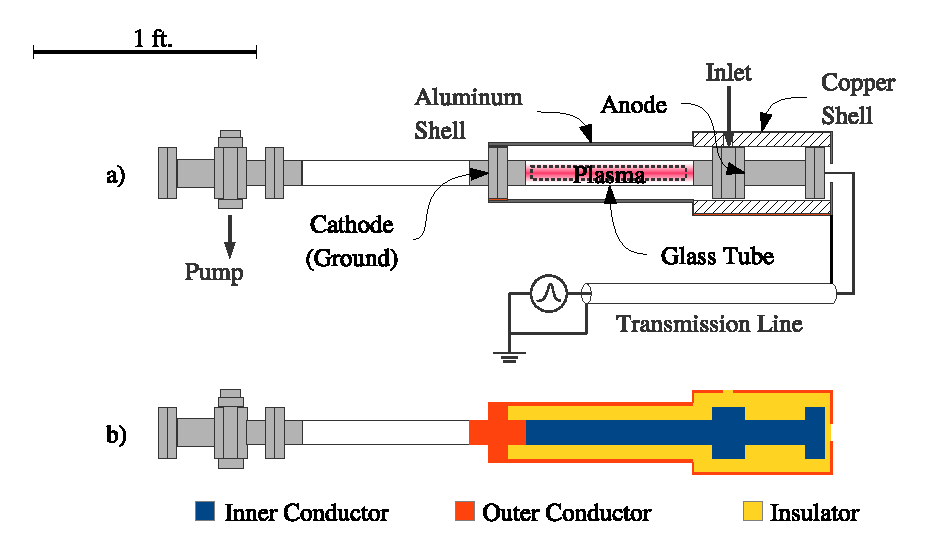
\includegraphics{./chapters/experiment/figures/appschem.eps}
  \caption{Two illustrations of the \acs{rpnd} apparatus. The upper version is
    an annotated sketch of the device, and the bottom version simplifies the
    geometry into its three electrical components.}
  \label{fig:appschem}
\end{figure}
Following from right to left, the inner conductor was composed of a vacuum
window, a nipple, a double-sided flange tapped for an NPT connection, and the
discharge tube containing the \acs{rpnd}. Unless otherwise noted, all vacuum
components featured DN35 CF flanges with copper gaskets.

The tube was composed of borosilicate glass with metal vacuum flanges on both
ends. The flanges of the tube also acted as the electrodes for the generation of
the \acs{rpnd}. The glass tube had an inner diameter of 3.3 cm, an outer
diameter of 4.0 cm, and a length of 22.9 cm. The overall length of the tube
including the flanges was 30 cm. In the figure shown here, the right electrode
served as the anode, and the left electrode was the cathode.

The dielectric surrounding the inner conductor was composed of several
components. The vacuum window, nipple, double-sided flange, and anode were
separated from the outer conductor by an air gap and a polytetrafluoroethylene
(\acs{ptfe}) tube, 20 cm in length with an inner diameter of about 7.5 cm, and
an outer diameter of 10 cm. The \acs{rpnd} portion of the inner conductor was
separated from the outer conductor by the glass tube and an air gap of about
2.54 cm.

The left side of the discharge tube, or cathode, connected to the outer
conductor and served as part of the current return path. Directly attached to
the cathode was an alumninum tube, held in place by an acetyl resin shaft collar
and a copper shim. Radial optical access to the discharge was provided by two
slots milled into the ground shell. The slots were positioned on opposite sides
of the shell and were 3.8 by 25.4 cm in length. The tube itself was 30 cm in
length.

The end of the aluminum tube nearest the anode was affixed to a copper sheet
which was oriented perpendicular with respect to the tube's axis of rotation.
The sheet was 10 cm square, and was attached to the tube with conductive copper
tape. A 5 cm diameter hole was cut into the copper sheet to allow the discharge
tube to pass through it. The sheet was secured to the edge of the \acs{ptfe}
tube by nylon screws. Surrounding the \acs{ptfe} tube was a second shell, made
of rolled copper sheet. This was electrically connected to the aluminum tube by
a braided copper strap. The right end of the \acs{ptfe} tube was covered by a
second copper sheet, 10 cm square. Again, the sheet was secured to the
\acs{ptfe} tube by nylon screws and in electrical contact with the copper shell.
In the center of the copper sheet was a HN bulkhead adapter for connection to
the transmission line. The inner conductor of the bulkhead adapter was connected
by a straight run of 5 cm of silicone-coated wire to the vacuum window flange.
The outer conductor of the bulkhead adapter provided the ground connection for
the discharge apparatus.\footnote{Measurements confirmed that the entirety of
the outer conductor had a low DC impedance to ground. However, it is likely that
at frequencies relevant to the \acs{rpnd}, the impedance is not negligible. As a
result, the outer conductor likely floats to a finite voltage during operation.}

The voltage pulse was generated by a \acs{fid} power supply, supplied by ANVS,
Inc. (model PT510NM). The amplitude of each pulse was fixed at 6.4 kV with a
repetition rate of 1.0 kHz. Each pulse had a fixed width of 25 ns, required
approximately 4 ns to rise from 10\% of its peak to 90\% of its peak, and was
roughly Gaussian in shape. A SRS DG645 delay generator was used to trigger the
power supply output for all experiments and provided a reference time base for
all measurements.

Preliminary experiments revealed multiple reflections between the power supply
and the anode. A long run of RG 213 coaxial cable was used to temporally
separate the reflections. This made it possible to study the effects of
individual pulses. Based on the length of the cable (about 13.7 m), the delay
was predicted to be 69.2 ns. As the reflection would have to cross the length of
the transmission line twice before it reached the anode again, the total
separation time between the initial pulse and each subsequent reflection was
predicted to be 138.4 ns. This calculated delay was found to closely match the
measured time period between the incident and reflected pulse.

\begin{figure}
  \centering
  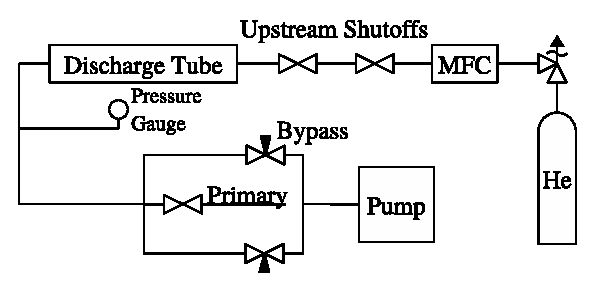
\includegraphics{./chapters/experiment/figures/pump.eps}
  \caption{Simplified diagram of the gas flow path and pumping system.}
  \label{fig:pump}
\end{figure}
A simplified version of the gas flow system can be seen in
figure~\ref{fig:pump}. The gas supply was provided by a bottle of ultra-high
purity helium. Following the regulator, the helium passed through a digital flow
controller which was set at 25.0 sccm for all experiments. The helium then
entered a gas distribution manifold, followed by a shutoff valve, a short run of
1/4" stainless steel tubing, another shutoff valve, about 2 m of 1/4"
polyethylene tubing, and then the discharge tube via the double-sided flange. 

The gas exited the discharge tube via an identical tube, on the side opposite
the inlet, see figure~\ref{fig:appschem}. This second tube was intended to
electrically isolate the discharge portion of the apparatus so that only a
single conductive path to ground existed. The pressure was monitored downstream
of the second tube with two capacitance manometers (one with a full scale range
of 10 Torr, the other with a range of 100 Torr). The gas exhaust of the second
tube was connected to an oil-seal roughing pump via three independent paths. The
primary pump path had the highest gas conductance and was controlled by a
bellows valve. However, this path was typically closed in favor of two needle
valve bypasses. The needle valves were used to control the pumping speed and
obtain the desired operating pressure. Immediately upstream of the roughing pump
was a zeolite trap in order to limit oil backstreaming.

The base pressure of the system was measured to be approximately 15 mTorr. The
leak rate was measured several times by evacuating the apparatus and then
sealing it from the pump by all three pump paths. The leak rate was found to be
$2.0\times 10^{-3}$ sccm. Given a constant flow rate of 25.0 sccm, the
fractional impurity can be conservatively estimated to be 80 ppm.

The assembled discharge apparatus can be seen in figure~\ref{fig:appphoto}.
\begin{figure}
  \centering
  \setlength\fboxsep{0pt}
  \setlength\fboxrule{1.0pt}
  \fbox{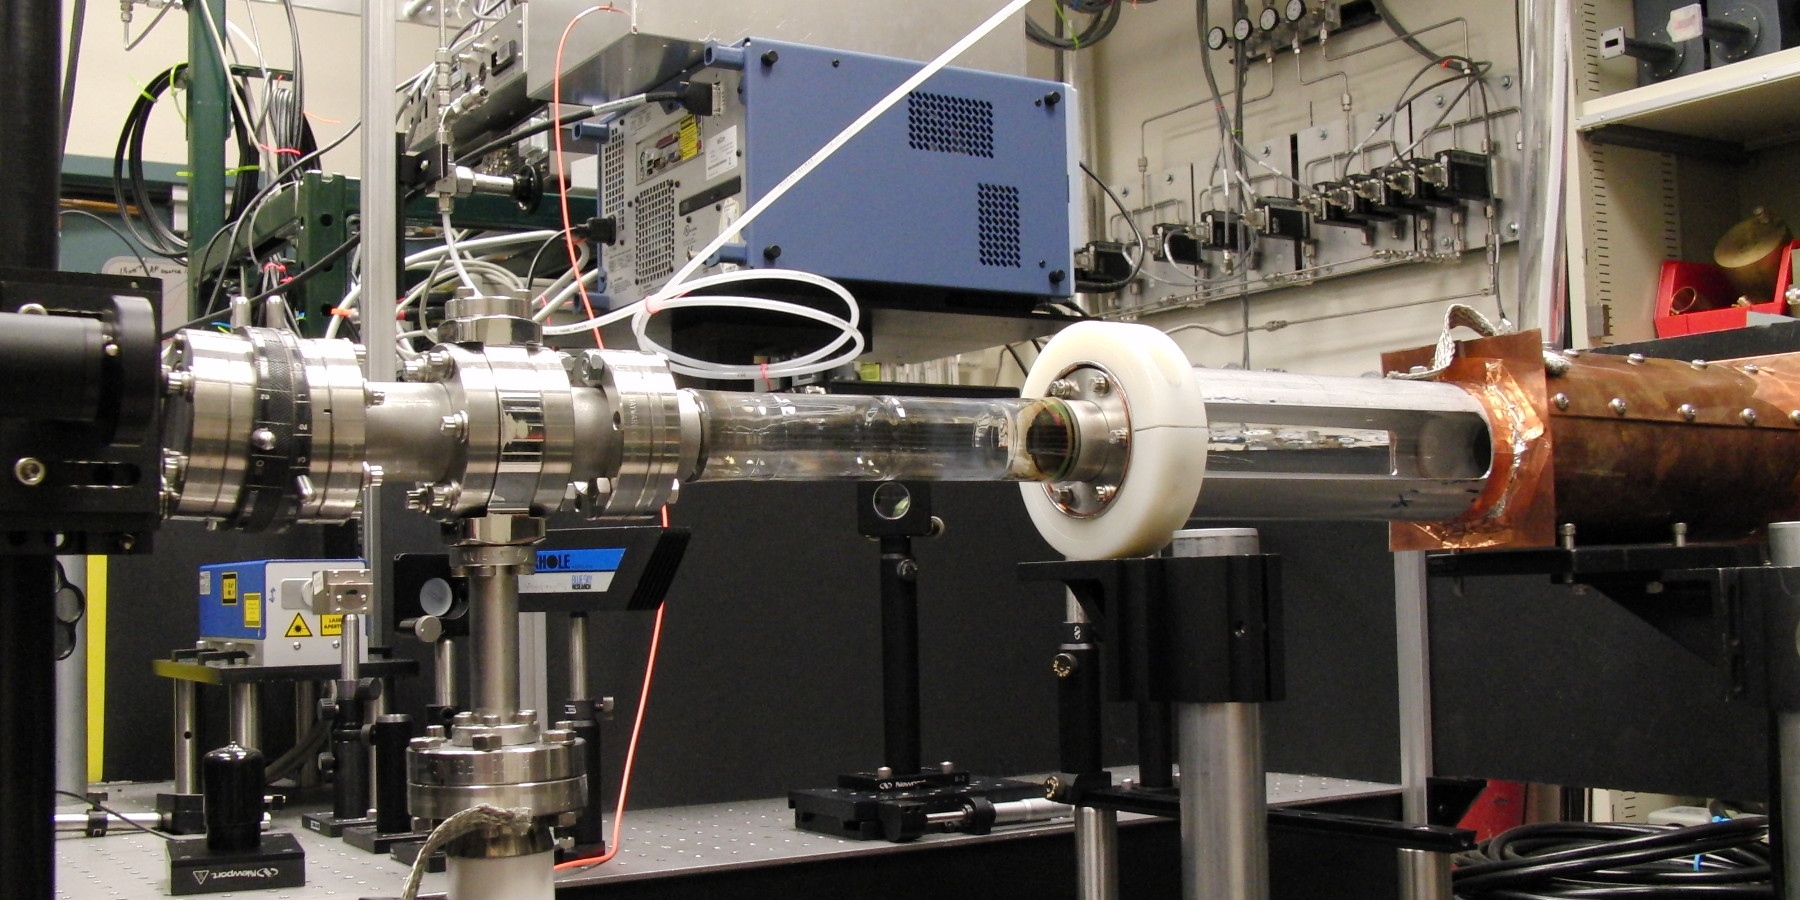
\includegraphics{./chapters/experiment/figures/appphoto.jpg}}
  \caption{Photograph of the discharge apparatus.}
  \label{fig:appphoto}
\end{figure}
The \acs{rpnd} apparatus was supported two 1.5 in mounting posts with angle
brackets. The mounting posts attached to a 122 cm by 76 cm optical breadboard,
supported by urethane shock absorbers, and a rigid frame. The roughing pump was
attached to the apparatus with flanged bellows in order to reduce mechanical
vibrations.

All electrical measurements were made with a LeCroy 6100A WaveRunner
oscilloscope which had a bandwidth of 1.0 GHz. Electrical connections to the
oscilloscope were made with RG 50/U coaxial cable and standard BNC connectors.
All connections were terminated at 50 $\Omega$ unless otherwise noted. The
voltage of the pulses was monitored from a $1:1000$ divider built into the power
supply. The current was measured from a current shunt which crossed a small
electrical break in the outer conductor of the transmission line. The shunt was
built into the transmission line as close as possible to the power supply, about
3 cm from the output connector.

The current shunt was composed of nine, low inductance, $1.0 \Omega$ resistors
connected in parallel. As illustrated in figure~\ref{fig:cbcs}
\begin{figure}
  \centering
  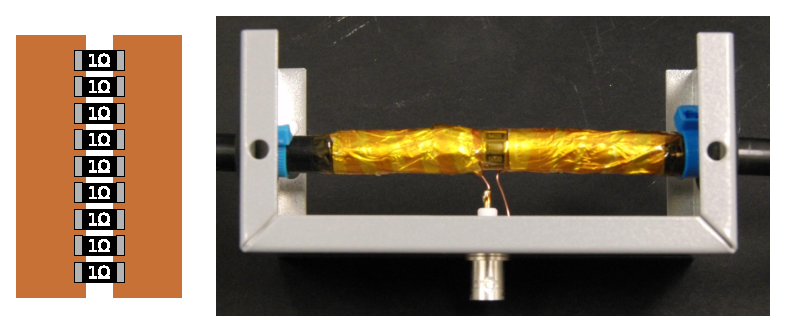
\includegraphics{./chapters/experiment/figures/cbcs.eps}
  \caption{Sketch of the unassembled back-current shunt, and a photograph of it
  assembled around the transmission line.}
  \label{fig:cbcs}
\end{figure}
the resistors were soldered to two strips of copper foil. This assembly was then
wrapped around the electrical break in the transmission line, bridging it. Two
short lengths of No.\ 18 copper wire were soldered to each side of the shunt
assembly. These were then attached to a BNC bulkhead connector, fitted to a
metal project box. The voltage across the resistors was used to measure the
current traveling through the outer conductor of the transmission line. The
copper foil was then secured to the outer conductor with several wraps of
aluminum foil, followed by a layer of polyimide tape.

Data were retrieved from the oscilloscope with a desktop computer via the GPIB
interface. Instrument control, data acquisition, and data storage were all
managed by a LabView program. Analog input and output was handled with the
auxiliary input and output ports of a SRS SR850 DSP lock-in amplifier.

\section{Field Calculations}

The electric field characteristics of the discharge apparatus were analyzed
using Ansoft Maxwell 9, a two-dimensional, electrostatic solver. At the top of
figure~\ref{fig:cfields}
\begin{figure}
  \centering
  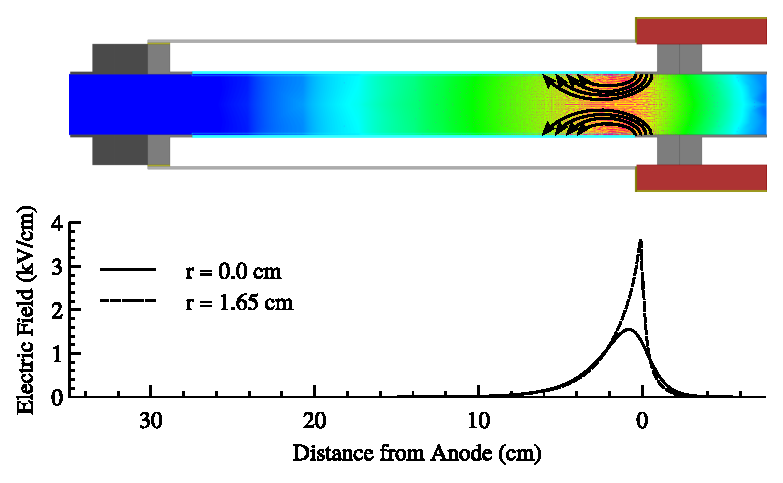
\includegraphics{./chapters/experiment/figures/cfields.eps}
  \caption{Heatmap and vector plot of the electric field in the \acs{rpnd}
  discharge apparatus.}
  \label{fig:cfields}
\end{figure}
is a logarithmic heatmap of the electric field magnitudes within the device.
Overlaid are the electric field vectors in magenta. Below this is a plot of the
electric field on a linear scale, across the central axis of the apparatus and
along the outer edge, adjacent to the glass tube. It is apparent that the field
strength is the strongest at the triple point which occurs near the glass-metal
seal. Also noticeable is the fast fall off of the electric field with distance
from the anode. The presence of the external ground shield produces an electric
field contour vastly different from that of two parallel plates. This is also
reflected in the electric field vectors. Specifically, the many locations
possess fields with strong radial components, especially those near the anode.

These static fields are only valid in the absence of free charge within the
system. However, these characteristics suggest that the discharge formation will
be somewhat different than the one-dimensional description of a streamer in
Chapter~\ref{chp:theory}. First, assume that the electrons are distributed
uniformly throughout the discharge tube, prior to the pulse. As a pulse is
applied, ionization would preferentially take place near the anode. As the
electrons would be drawn toward the anode, and leave behind some amount of
positive space charge. However, as the positive space charge builds up, it would
begin to act as a virtual anode, increasing the electric field further from the
physical anode. The virtual anode would then begin to draw its own electron
current, predominantly from around the edges, near the wall. In this manner, the
discharge would propagate away from the anode, leaving a quasineutral ionized
gas in the center of the discharge tube and a positive space charge region along
the wall.

\section{Operating Procedures}

One of two operating procedures for the \acs{rpnd} was used depending on how
recently the discharge had last been turned on. If the discharge was inactive
for over one hour, then a full startup procedure was used. Otherwise, an abbreviated
process was used.

In the case that the discharge had not been operated for over an hour, the
roughing pump was turned on and the primary pump path valve was opened as was
the first shutoff valve upstream of the discharge chamber, seen in
figure~\ref{fig:pump}. The system was then allowed to pump down to its base
pressure. Afterward the second upstream shutoff valve was opened and the system
was again allowed to reach base pressure. At this point the helium flow was
turned on and set to 25.0 sccm. The primary pump path was then closed and the
needle valve bypasses were used to adjust the system pressure to 3.0 Torr.

Next, the delay generator was turned on and the output for triggering the power
supply was activated. Then, the \acs{fid} power supply was turned on. This would
produce an easily visible discharge within the discharge tube. The system was
allowed to operate at this condition for one hour in order to remove potential
contamination on the walls and electrodes. At the end of this period, the
voltage waveform was checked to ensure that it was consistent with previous
experiments. Once this was confirmed, the pressure was adjusted to the desired
operating condition.

The discharge was shutdown by first shutting off the power supply, followed by
the delay generator. Then, the helium flow was shut off, and the primary pump
path was opened. The system was allowed to come to base pressure before the two
upstream shutoff valves were closed, after which the primary pump path was
closed. The roughing pump was then shut off.

In the cases that the discharge had been operated within the last hour, it was
possible to use an abbreviated startup procedure. This process was fundamentally
the same as the previous one, however once the pump-related procedures were
complete the discharge only required five minutes to reach a steady state. This
was verified with multiple measurements of the current and voltage
characteristics as well as the discharge emissions. At times prior to this five
minute equilibration period, the reflected pulse energy was noticeably higher,
and the delay between the trigger pulse and the output pulse was variable.

It seems likely that the increased reflected pulse energy during the
equilibration period is due to poor matching between the output impedance of the
power supply and the plasma load \cite{Pancheshnyi2006}. When the pulse train is
initiated, the first series of pulses perceive an almost open load. During this
time, the plasma density tends to increase more with each pulse than is lost
between pulses. This increase in plasma density, reduces its impedance and
improves energy coupling to the plasma. At the same time, the increasing plasma
density results in an increasing shielding effect of the applied voltage.
Eventually, these effects balance out and the density increased caused by each
pulse equals the density decrease which occurs between pulses. At this point the
energy coupled into the plasma with each pulsed remains essentially fixed.

\section{Electrical Characteristics}

The typical voltage waveform, as seen in figure~\ref{fig:waveform},
\begin{figure}
  \centering
  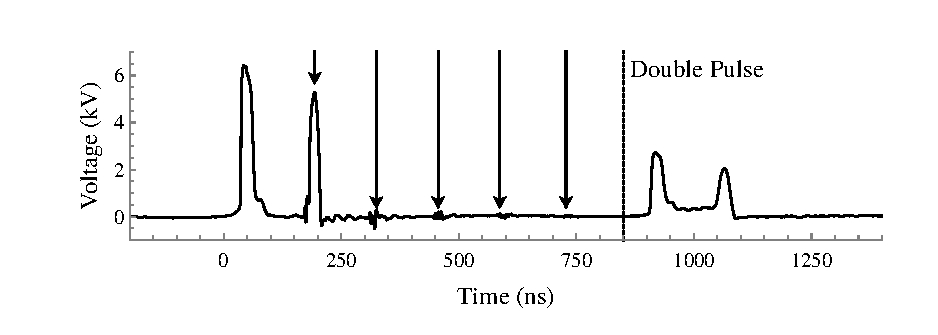
\includegraphics{./chapters/experiment/figures/waveform.eps}
  \caption{Typical voltage waveform of the \acs{rpnd}. Arrows indicate
    reflections back to the power supply. The dotted line delineates the time at
    which the power supply begins to exhibit double pulsing.}
  \label{fig:waveform}
\end{figure}
exhibited a number of features. It begins with an incident pulse at $t = 0.0$.
138 ns later, it is followed by the pulse that has been reflected from the
anode. The reflected pulse is somewhat smaller, proportional to the energy
deposited in the discharge. Additional reflections are visible at integer
multiples of 138 ns. These subsequent reflections are much smaller than the
initial one, suggesting that much of the remaining pulse energy was dissipated
after the first reflection reached the anode. Curiously, a second pulse appears
at 800 ns. This is believed to be a peculiarity of the power supply. For the
most part, analysis of the \acs{rpnd} will focus on the times which precede 280
ns (the incident pulse and first reflected pulse).

The properties of the \acs{rpnd} were examined at: 0.3, 0.5, 1.0, 2.0, 3.0, 4.0,
8.0, and 16.0 Torr. The appearance of the discharge varied with the pressure in
a continuous fashion, however it was apparent that there were three regimes of
operation. At the low pressures, 0.3 and 0.5, it was difficult to initiate the
discharge. Often, it would be necessary to increase the pressure to initiate the
discharge, and then reduce the pressure to the desired conditions. The discharge
appeared dim and relatively constricted about the central axis of the discharge
tube, with a radial extent of approximately 1 cm. Accompanying these pressures
was a large degree of electronic noise. This manifested primarily in the current
waveforms, as seen in figure~\ref{fig:waveforms},
\begin{figure}
  \centering
  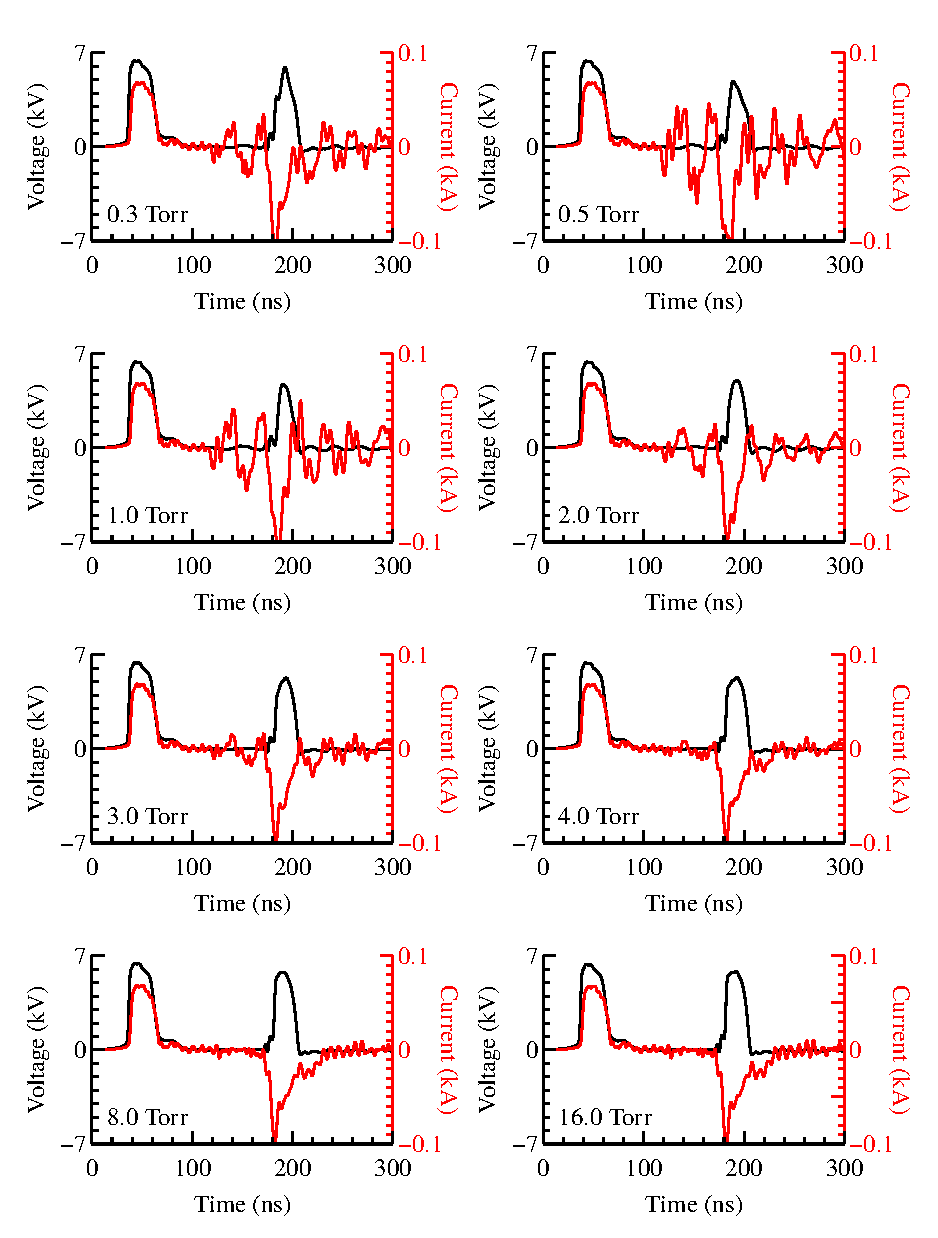
\includegraphics{./chapters/experiment/figures/waveforms.eps}
  \caption{High resolution views of the voltage and current waveforms for the
  first incident and reflected pulse, at each of the operating pressures.}
  \label{fig:waveforms}
\end{figure}
as well as a number of equipment malfunctions.

As the pressure was increased (from 1.0-4.0 Torr), the electrical noise was
observed to subside. The current waveforms showed significant reductions in the
ringing that was particularly prominent at lower pressures. In addition, the
visual extent of the discharge increased substantially, to the point where it
could be considered volume-filling. The discharge also increased its axial
extent as well, eventually reaching well past its intended limit at the cathode.
This occurred despite attempts to isolate the downstream pump sections from the
discharge. 

Such behavior is similar to that observed in plasma bullets \cite{Lu2006} where
the discharge is able to continue far past the cathode. This suggests that
development of the \acs{rpnd} along the discharge tube led by a large region of
positive space charge, as suggested in the discussion of the field
characteristics. The ions that produce this positive space charge are eventually
collected at the cathode or neutralized at the walls, however their low mobility
(as noted in Chapter~\ref{chp:theory}) prevents this from happening on time
scales relevant to the \acs{rpnd} formation.

At higher operating pressure (8.0 and 16.0 Torr), the discharge receded back
toward the cathode. This was accompanied by a decrease in the apparent
brightness of the discharge to levels similar to that of the low pressure
conditions. In contrast, the discharge appeared to remain volume-filling. While
discharge initiation was difficult at the higher pressures, it was not
accompanied by the electrical noise observed at lower pressures.

\section{Energy Coupling}

The product of the voltage and current waveforms, as seen in
figure~\ref{fig:waveforms}, gives the power deposited in the discharge as a
function of time. Subsequently, the power integrated over time gives the total
energy deposited in the discharge. However, this approach is somewhat
complicated by several features of the \acs{rpnd}. As previously mentioned, the
pulses produced by the power supply are not completely absorbed by the
discharge. Therefore, the integration must be carried out over both the incident
and the reflected pulse. Additionally, there is the concern that the
oscillations in the current measurements could introduce fluctuations in the
calculated energy deposition. However, the small voltage signal limits the error
introduced by these fluctuations to less than 1\%.

Figure~\ref{fig:energies}
\begin{figure}
  \centering
  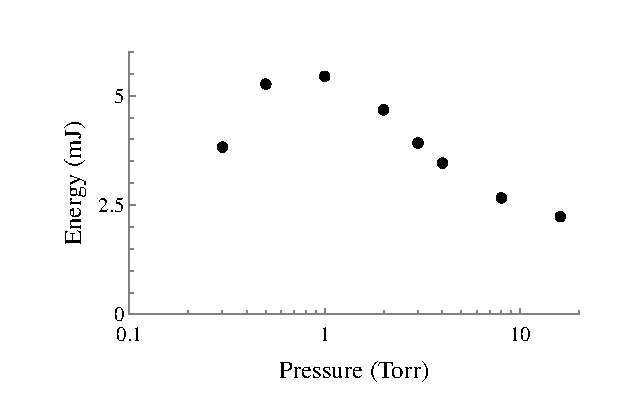
\includegraphics{./chapters/experiment/figures/energies.eps}
  \caption{Plot of the energy coupled into the discharge with the first pulse as
  a function of pressure.}
  \label{fig:energies}
\end{figure}
gives the total energy deposited for the first pulse at each of the operating
conditions. The energy coupled to the discharge peaks at an energy of 5.5 mJ
(out of a total incident energy of 8.8 mJ) at a pressure of 1.0 Torr, after
which it slowly decreases. This peak in the coupled energy is coincident with
the peak brightness of the discharge. Together, these suggest that the density
of excited states will be optimized at intermediate pressures.

Though there appear to be no direct comparisons available in the literature,
several papers report on energy coupling for similar systems. Macheret,
Schneider, and Murray studied a parallel plate \acs{rpnd} in air, at 1-10 Torr
and reported a total energy deposition of 0.30-0.36 mJ, increasing with pressure
\cite{Macheret2006}. Nishihara et al.\ recorded values of 1-2 mJ in a nitrogen
\acs{rpnd} \cite{Nishihara2006}. Pancheshnyi et al., in the study of an
air-propane mixture at 750 Torr, found that each pulse deposited about 1.9 mJ of
energy. Overall, the measured values for the deposited energy appear to be in
comparable with those previously measured.

From an applications standpoint, the potential existence of a condition which
optimizes the production of excited states is an interesting one. This behavior
is also compelling from a physical standpoint as it suggests a phase change in
the competition of two or more processes. Though this kind of competition is
reminiscent of Paschen's law, the duration of the pulse is too short for
appreciable ion drift to occur (an estimated maximum of 3 mm), therefore
secondary electron emission is not important. These observations provide further
impetus for a close examination of the \acs{rpnd} properties, particularly the
excited state dynamics.
